\chapter{Tuning the Models}

\section{Inertial Circles in the Dynamic Model}

\begin{figure}
    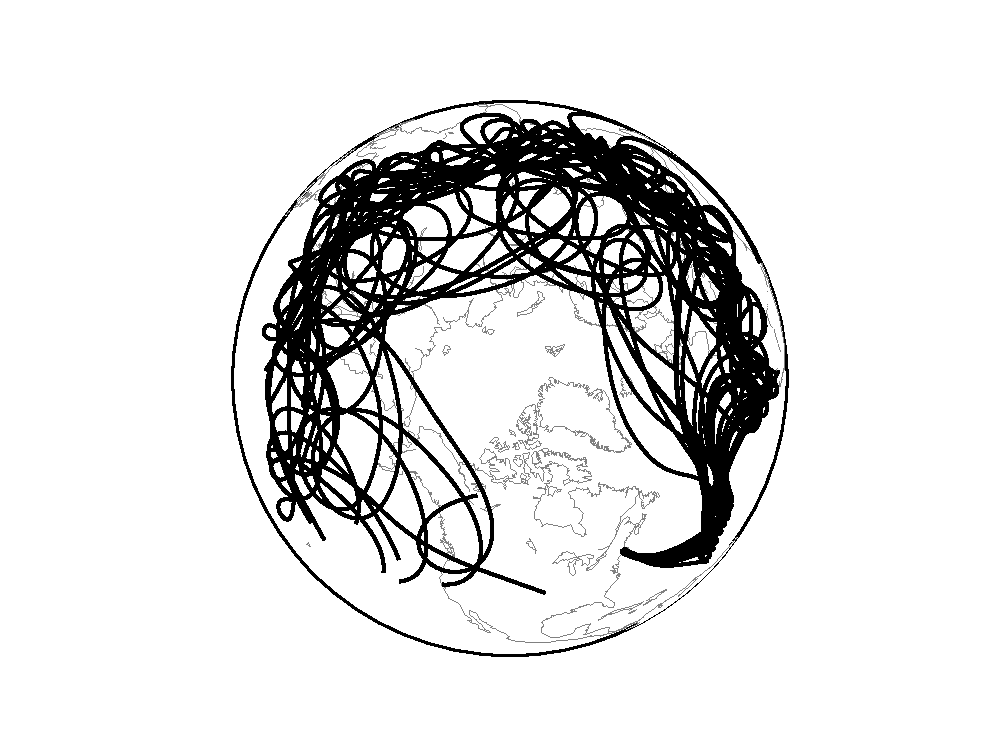
\includegraphics[width=\textwidth]{force_180.eps}
    \caption{Twenty five dynamic trajectories launched in an evenly-spaced grid with its lower-left corner at 41, -72 and upper-right corner at 42, -71. 
    The large spirals are implausible for jet stream flow and reflect a problem with the model.}
    \label{fig:force_180}
\end{figure}

\section{Adding Friction to the Dynamic Model}

[[[Inertial circles have been encountered before in dynamic models and there are different ways of dealing with them.]]] \cite{stohl_accuracy_1998}
One approach, used by Stohl and Seibert, is to take a weighted average of the wind speeds from the dynamic model and interpolated speeds from a kinematic model at each timestep.
Another approach is to change the frictionless assumption of the dynamical model.
[[[Why does the force of friction damp oscillations?]]]
Using the definition of geostrophic wind in Equations \ref{eq:u_g} and \ref{eq:v_g}, Equations \ref{eq:uvelocitygeo} and \ref{eq:vvelocitygeo} with an added friction term become

\begin{align}
    \frac{du}{dt} &= f (v - v_g) - r_f (u - u_g) \\
    \frac{dv}{dt} &= -f (u - u_g) - r_f (v - v_g).   
\end{align}

The friction parameter $r_f$ is analogous to the Coriolis parameter: it has units of second$^{-1}$ and is a measure of the force of friction.

\section{Choosing a Timestep} \label{sec:timestep}

\begin{figure}[t!]
    \begin{subfigure}[t]{0.5\textwidth}
    	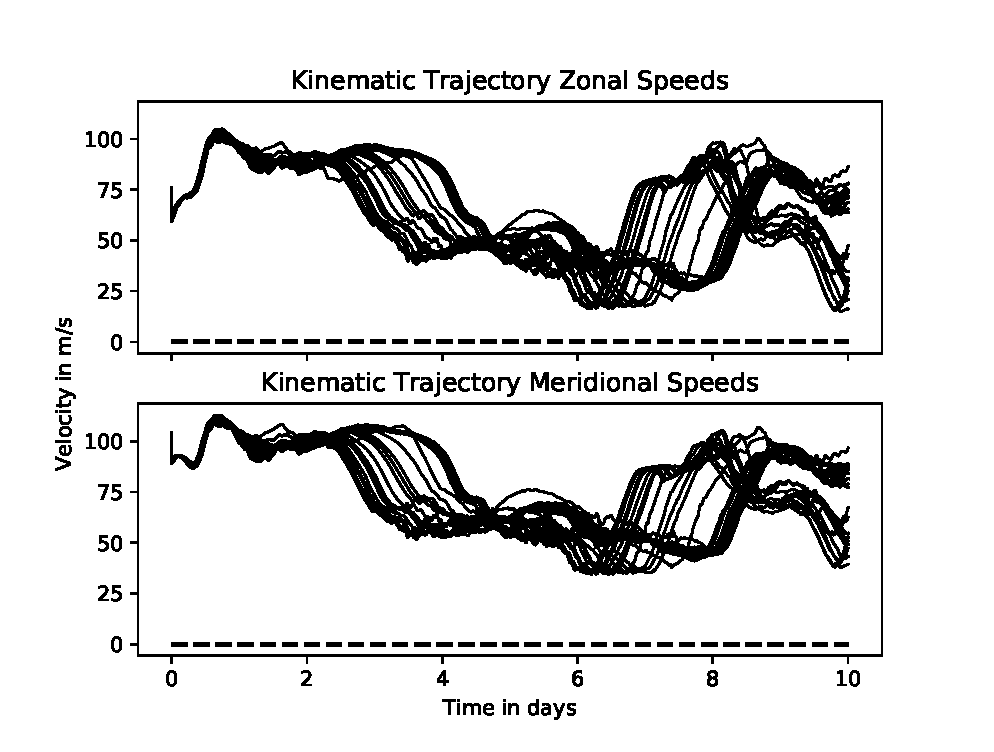
\includegraphics[width=\textwidth]{timestep_grid_180.eps}
    \end{subfigure}
    ~
    \begin{subfigure}[t]{0.5\textwidth}
        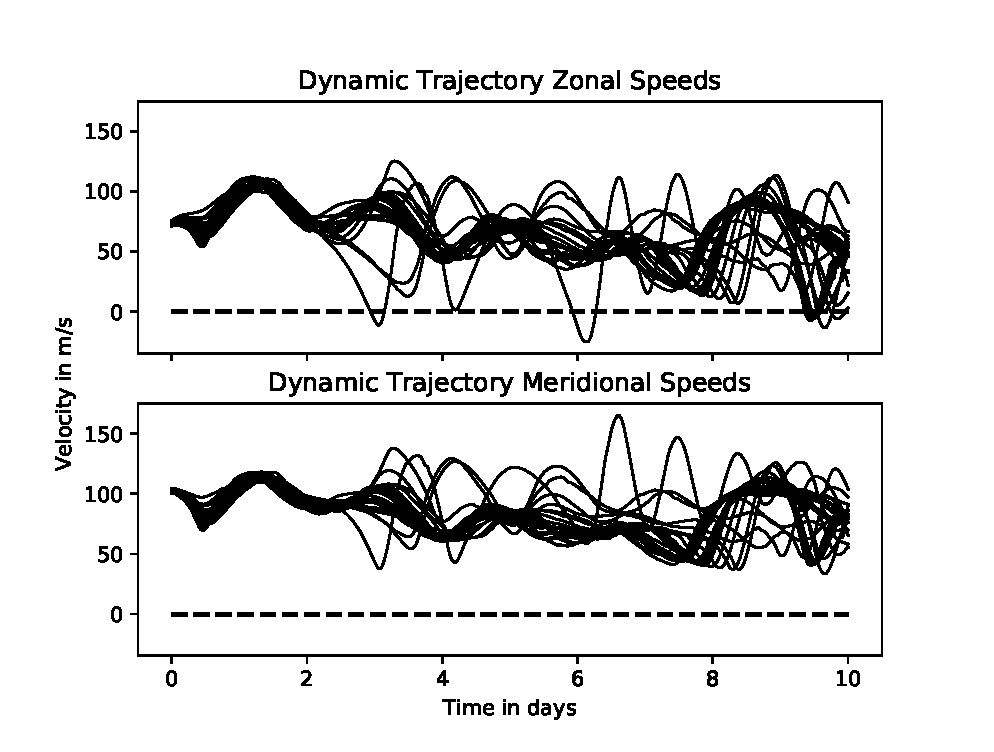
\includegraphics[width=\textwidth]{timestep_friction_180.eps}
    \end{subfigure}
\end{figure}
